% Thanks to Dan Wang for the Beamer template!

\documentclass[9pt]{beamer}

% Fill in variables below %
% ++++++++++++++++++++++++++++++++++++++++++++++++++++++++++++++++++++++++ %
\newcommand{\thesemester}{Spring 2012}
\newcommand{\themidterm}{CS 61B Midterm 2 Review}
\newcommand{\theauthors}{Lu Cheng, Harrison Wallace,  Riyaz Faizullabhoy, John Du}
\newcommand{\theorganization}{Eta Kappa Nu, Mu Chapter \\
University of California, Berkeley}
\newcommand{\thedate}{November 3 2012}
\newcommand{\thelanguage}{Java}
% ++++++++++++++++++++++++++++++++++++++++++++++++++++++++++++++++++++++++ %

% Preamble %
% ------------------------------------------------------------------------ %
\usepackage{url}
\usepackage{relsize}
\usepackage{color}
\usepackage{listings}
\usepackage{multirow}
\usepackage{array}
\usepackage{bm}
\usepackage{framed}
\usepackage{tikz}
\usepackage{mathtools}
\DeclarePairedDelimiter{\ceil}{\lceil}{\rceil}
\DeclarePairedDelimiter{\floor}{\lfloor}{\rfloor}
\usetikzlibrary{trees}
\usetikzlibrary{shapes.geometric}
\usetikzlibrary{shapes.misc}
\usetikzlibrary{shapes.multipart}
\usetikzlibrary{positioning}

% Listings Package %
\usepackage{listings}
\lstset{numbers=left,
    numberstyle=\tiny,
    showstringspaces=false,
    frame=leftline,
    language=Python,
    escapeinside=\$\$,
    keywordstyle=\color{blue},
    xleftmargin=20pt,
    morecomment=[l]{//},
    }

\usetheme{Singapore}
\setbeamertemplate{mini frames}[circle]
\setbeamertemplate{footline}[frame number]

\title{\themidterm}
\author{\theauthors}
\institute{\theorganization}
\date{\thedate}
% ------------------------------------------------------------------------ %

\begin{document}

% Title Page %
% ------------------------------------------------------------------------ %

\begin{frame}
  \titlepage
\end{frame}

% Asymptotic Analysis %
% ------------------------------------------------------------------------ %
\section{Asymptotic Analysis}
\subsection{Asymptotic Analysis}

\begin{frame}[fragile]{True/False}
  Determine the truth value of the following statement:

  \[n^2 \in \Omega(n!)\]

  \begin{enumerate}
    \item
      True
    \item
      \alert<2>{False}
  \end{enumerate}
\end{frame}

\begin{frame}[fragile]{True/False}
  Determine the truth value of the following statement:

  \begin{quote}
    A {\bf preorder} traversal of a binary search tree will visit the nodes
    in {\bf ascending} order of their keys.
  \end{quote}

  \begin{enumerate}
    \item
      True
    \item
      \alert<2->{False}
  \end{enumerate}

  \uncover<3>{\begin{framed}
    An {\bf inorder} traversal of a BST will visit the nodes in ascending
    order.
  \end{framed}}
\end{frame}

\begin{frame}[fragile]{Algorithmic Analysis}
What are the bounds of the following algorithm? \\
\uncover<2->{\alert<2>{O($n$), where $n$ is the size of {\tt toAdd}.}}\\
{ \small
\begin{lstlisting}
public ArrayList<String> convertToArrayList(String[] toAdd) {
    int N = toAdd.length;
    ArrayList<String> result = new ArrayList<String>(0);
    for (String x : toAdd) {
         result.add(x);
    }
    return result;
}
  \end{lstlisting}
  }
\end{frame}

\begin{frame}[fragile]{Algorithmic Analysis}
What are the bounds of the following algorithm? \\
\uncover<2->{\alert<2>{O($n$), where $n$ is the size of {\tt A}.}}\\
{
\begin{lstlisting}
public void reverse(LinkedList<String> A) {
    int N = A.size();
    for (int i = 0; i < N; i++) {
        String last = A.removeLast();
        A.addFirst(last);
    }
}
  \end{lstlisting}
  }
\end{frame}

\begin{frame}[fragile]{Algorithmic Analysis}
What are the bounds of the following algorithm? \\
\uncover<2->{\alert<2>{O($n^2$), where $n$ is the size of {\tt A}.}}\\
{
\begin{lstlisting}
public void reverse(ArrayList<String> A){
    int N = A.size();
    for(int i = 0; i < N; i++){
        String last = A.remove(N - 1);
        A.add(0, last);
    }
}
  \end{lstlisting}
  }
\end{frame}

\begin{frame}[fragile]{Algorithmic Analysis}
What are the bounds of the following algorithm? \\
\uncover<2->{\alert<2>{O($n$), where $n$ is the size of {\tt toSort}.}} \\
{ \footnotesize 
\begin{lstlisting}
public ArrayList<Integer> bucketNums(ArrayList<Integer> toSort){
    int N = toSort.size();
    HashMap<Integer, Integer> occurences 
        = new HashMap<Integer, Integer>();
    for(int x : toSort){
        if(!occurrences.containsKey(x)){
            occurrences.put(x, 1);
        } else {
            occurrences.put(x, occurrences.get(x) + 1;
        }
    }
    ArrayList<Integer> sorted = new ArrayList<Integer>();
    for(int key : occurrences.keySet()){
        for (int i = 0; i < occurences.get(key); i++){
            sorted.add(key);
        }
    }
    return sorted;
}
  \end{lstlisting}
  }
\end{frame}


% Trees %
% ------------------------------------------------------------------------ %
\section{Trees}
\subsection{Binary Search Trees}
\begin{frame}[fragile]{Binary Search Trees: Review}
  A binary search tree is a tree with the following properties:
  \begin{itemize}
    \item
      The tree is a binary tree (each node has at most two children).
    \item
      The left subtree of any node contains only keys less than that node's
      key
    \item
      The right subtree of any node contains only keys greater than that
      node's key
  \end{itemize}

  \uncover<2>{
  To {\tt find} an element $e$:
  \begin{enumerate}
    \item
      Start at the root. If the tree is empty, then the key is not in the
      tree.
    \item
      If the root's key is $e$, then return the value. Otherwise:
      \begin{enumerate}[1.]
        \item
          If the root's key is greater than $e$, then run {\tt find()}
          on its left child.
        \item
          Otherwise, run {\tt find()} on its right child.
      \end{enumerate}
  \end{enumerate}
  }
\end{frame}

\begin{frame}[fragile]{Binary Search Trees: Review}
  To {\tt insert()} an element, traverse the tree like {\tt find()}
  until an empty tree is reached. Insert the element into that spot.

  \vspace{2em}

  \uncover<2->{
  To {\tt remove()} an element:
  \begin{enumerate}
    \item
      Search for the item using {\tt find()}.
      \begin{enumerate}[1.]
        \item
          If it has 0 children, remove the node from the tree.
        \item
          If it has 1 child, replace the node with its child.
        \item
          If it has 2 children, replace the label of the node with the label
          of its in-order successor and remove that node.
      \end{enumerate}
  \end{enumerate}
  }

  \uncover<3->{
  \begin{framed}
    The {\bf in-order successor} of a node is the node that is visited after
    the first node in an in-order traversal of the tree. In a binary search
    tree, the label of the in-order successor is the smallest value that is
    greater than the node's label. The in-order successor of a node is the
    bottom leftmost child in its right subtree.
  \end{framed}
  }
\end{frame}

\subsection{Problems}

\begin{frame}[fragile]{Binary Search Trees}
  Given the following binary search tree:

  \tikzstyle{level 1}=[level distance=3em, sibling distance=8em]
  \tikzstyle{level 2}=[level distance=3em, sibling distance=4em]
  \tikzstyle{node} = [circle, draw, text width=1em]

  \begin{tikzpicture}[grow=down]
    \node[node] {7}
      child {
        node[node] {3}
          child {
            node[node] {1}
          }
          child {
            node[node] {6}
          }
      }
      child {
        node[node] {9}
          child {
            node[node] {8}
          }
          child {
            node[node] {12}
          }
      };
  \end{tikzpicture}

  Draw what it looks like after each of the following consecutive method
  calls:
  \begin{itemize}
    \item
      {\tt insert(5)}
    \item
      {\tt remove(3)}
    \item
      {\tt insert(3)}
    \item
      {\tt remove(9)}
  \end{itemize}
\end{frame}

\begin{frame}[fragile]{Binary Search Trees}
  \begin{columns}
    \begin{column}{0.5\textwidth}
      After {\tt insert(5)}:
      \vspace{1em}

      \uncover<2->{
      \tikzstyle{level 1}=[level distance=3em, sibling distance=8em]
      \tikzstyle{level 2}=[level distance=3em, sibling distance=4em]
      \tikzstyle{level 3}=[level distance=3em, sibling distance=3em]
      \tikzstyle{node} = [circle, draw, text width=1em]

      \begin{tikzpicture}[grow=down]
        \node[node] {7}
          child {
            node[node] {3}
              child {
                node[node] {1}
              }
              child {
                node[node] {6}
                  child {
                    node[node] {5}
                  }
                  child[missing] {}
              }
          }
          child {
            node[node] {9}
              child {
                node[node] {8}
              }
              child {
                node[node] {12}
              }
          };
      \end{tikzpicture}
      }

      After {\tt remove(3)}:
      \vspace{1em}

      \uncover<3-> {
      \begin{tikzpicture}[grow=down]
        \node[node] {7}
          child {
            node[node] {5}
              child {
                node[node] {1}
              }
              child {
                node[node] {6}
              }
          }
          child {
            node[node] {9}
              child {
                node[node] {8}
              }
              child {
                node[node] {12}
              }
          };
      \end{tikzpicture}
      }
    \end{column}
    \begin{column}{0.5\textwidth}
      After {\tt insert(3)}:
      \vspace{1em}

      \uncover<4-> {
      \tikzstyle{level 1}=[level distance=3em, sibling distance=8em]
      \tikzstyle{level 2}=[level distance=3em, sibling distance=4em]
      \tikzstyle{level 3}=[level distance=3em, sibling distance=3em]
      \tikzstyle{node} = [circle, draw, text width=0.8em]

      \begin{tikzpicture}[grow=down,scale=0.8]
        \node[node] {7}
          child {
            node[node] {5}
              child {
                node[node] {1}
                  child[missing] {}
                  child {
                    node[node] {3}
                  }
              }
              child {
                node[node] {6}
              }
          }
          child {
            node[node] {9}
              child {
                node[node] {8}
              }
              child {
                node[node] {12}
              }
          };
      \end{tikzpicture}
      }

      After {\tt remove(9)}:
      \vspace{1em}

      \uncover<5-> {
      \begin{tikzpicture}[grow=down,scale=0.8]
        \node[node] {7}
          child {
            node[node] {5}
              child {
                node[node] {1}
                  child[missing] {}
                  child {
                    node[node] {3}
                  }
              }
              child {
                node[node] {6}
              }
          }
          child {
            node[node] {12}
              child {
                node[node] {8}
              }
              child[missing] {}
          };
      \end{tikzpicture}
      }
    \end{column}
  \end{columns}
\end{frame}

\begin{frame}[fragile]{Binary Search Trees}
Given: \\
 {
  \begin{lstlisting}
public class Node{
    Node left, right, parent;
    int value;
}

public boolean isLeftChild(Node N){
    //Fill out here
}
  \end{lstlisting}
  }
Write a method {\tt isLeftChild} that determines if the {\tt Node N} is the left child of its parent.
\end{frame}

\begin{frame}[fragile]{Binary Search Trees}
Solution: \\
{
\begin{lstlisting}
public class Node{
    Node left, right, parent;
    int value;
}

public boolean isLeftChild(Node N){
    return (N.parent != null) && (N.parent.left == N);
}
  \end{lstlisting}
  }
\end{frame}

\begin{frame}[fragile]{Binary Search Trees}
Given: \\
 {
  \begin{lstlisting}
public class Node{
    Node left, right, parent;
    int value;
}

public boolean isParent(Node N){
    //Fill out here
}
  \end{lstlisting}
Write a method {\tt isParent} that determines if the {\tt Node N} is a parent.
  }
\end{frame}

\begin{frame}[fragile]{Binary Search Trees}
Solution: \\
 {
  \begin{lstlisting}
public class Node{
    Node left, right, parent;
    int value;
}

public boolean isParent(Node N){
    return (N.left != null) || (N.right != null);
}
  \end{lstlisting}
  }
\end{frame}

\begin{frame}[fragile]{Binary Search Trees}
Given: \\
 {
  \begin{lstlisting}
public class Node{
    Node left, right, parent;
    int value;
}

public boolean isMinOfTree(Node N){
    //Fill out here. Hint: you may need a helper method.
}
  \end{lstlisting}
Write a method {\tt isMinOfTree} that determines if the {\tt Node N} is the minimum element of the binary search tree that contains it. \\
  }
\end{frame}

\begin{frame}[fragile]{Binary Search Trees}
Solution: \\
 { \small
  \begin{lstlisting}
public class Node{
    Node left, right, parent;
    int value;
}

public boolean isMinOfTree(Node N){
    return N.left == null && isLeftChild(N)
        && isMinOfTreeHelper(N.parent);
}

public boolean isMinOfTreeHelper(Node N){
    return (N == null)
        || (isLeftChild(N) && isMinOfTreeHelper(N.parent));
}
  \end{lstlisting}
  }
\end{frame}


% Hashing %
% ------------------------------------------------------------------------ %
\section{Heaps}
\subsection{Theory}
\begin{frame}[fragile]{Heaps: Review}
  A heap is a binary tree with the following properties:
  \begin{itemize}
    \item
      The tree is complete. That is, every level is filled except possibly
      the last, which is filled from left to right.
    \item
      The {\em heap property} or {\em heap invariant} holds for all nodes of
      the tree: If $B$ is a descendant of $A$, then the key of $B$ is
      greater than or equal to that of $A$ (for a min heap).
  \end{itemize}

  \pause
  Heaps are usually implemented as arrays:

  \tikzstyle{level 1}=[level distance=3em, sibling distance=8em]
  \tikzstyle{level 2}=[level distance=3em, sibling distance=4em]
  \tikzstyle{level 3}=[level distance=3em, sibling distance=3em]
  \tikzstyle{node} = [circle, draw, text width=0.8em]

  \begin{tikzpicture}[grow=down,scale=0.8]
    \node [rectangle split, rectangle split parts=8, rectangle split
    horizontal, draw] at (0, -1) {
      $\times$
      \nodepart{two}3
      \nodepart{three}5
      \nodepart{four}4
      \nodepart{five}8
      \nodepart{six}7
      \nodepart{seven}6
      \nodepart{eight}9
    };

    \node[node] at (8, 0) {3}
      child {
        node[node] {5}
          child {
            node[node] {8}
          }
          child {
            node[node] {7}
          }
      }
      child {
        node[node] {4}
          child {
            node[node] {6}
          }
          child {
            node[node] {9}
          }
      };
  \end{tikzpicture}
\end{frame}

\begin{frame}[fragile]{Heaps: Review}
  To {\tt insert()} an element:
  \begin{enumerate}
    \item
      Insert the item at the end of the array.
    \item
      Bubble up by repeatedly swapping with parents until the heap property
      is satisfied.
  \end{enumerate}

  \vspace{2em}

  \pause
  To {\tt removeMin()}:
  \begin{enumerate}
    \item
      Swap the first and last elements of the array.
    \item
      Remove the last element and return it.
    \item
      Bubble the root down by repeatedly comparing with both of its children
      and swapping until the heap property is satisfied.
  \end{enumerate}
\end{frame}

\begin{frame}[fragile]{Heaps: Review}
        \begin{center}
        \scalebox{0.8}{
                \begin{tabular}{|c|c|c|c|}
                \hline
                \multicolumn{4}{|c|}{{\bf Running Times}} \\
                \hline
                & Binary Heap & Sorted List/Array & Unsorted List/Array \\
                \hline
                 min() & $\Theta(1)$ & $\Theta(1)$ & $\Theta(n)$ \\
                \hline
                insert() (worst case)     & $\Theta(log n)^{*}$ & $\Theta(n)$ & $\Theta(1)^{*}$ \\
                \hline
                insert() (best case)     & $\Theta(1)^{*}$ & $\Theta(1)^{*}$ & $\Theta(1)^{*}$ \\
                \hline
                removeMin() (worst case)     & $\Theta(log n)$ & $\Theta(1)$ & $\Theta(n)$ \\
                \hline
                removeMin() (best case)     & $\Theta(1)$ & $\Theta(1)$ & $\Theta(n)$ \\
                \hline
                \end{tabular}
        }
        \end{center}

        \begin{description}
                \item{*}
                If you are using an array-based data structure, these running times assume that you don't run out of room. If you do, it will take $\Theta(n)$ time to allocate a larger array and copy the entries into it. However, if you double the array size each time, the average running time will still be as indicated.
        \end{description}
\end{frame}


\subsection{Problems}

\begin{frame}[fragile]{Heaps}
  Starting with an empty {\bf max heap}, perform the following consecutive insertions:
  \begin{enumerate}
    \item
      {\tt insert(5)}
    \item
      {\tt insert(1)}
    \item
      {\tt insert(2)}
    \item
      {\tt insert(6)}
    \item
      {\tt insert(4)}
    \item
      {\tt insert(3)}
  \end{enumerate}

  Draw what the heap looks like after these values are inserted.

  \tikzstyle{level 1}=[level distance=3em, sibling distance=8em]
  \tikzstyle{level 2}=[level distance=3em, sibling distance=4em]
  \tikzstyle{level 3}=[level distance=3em, sibling distance=3em]
  \tikzstyle{node} = [circle, draw, text width=1em]

  \pause
  {\bf Answer:}

  \begin{tikzpicture}[grow=down]
    \node[node] {6}
      child {
        node[node] {5}
          child {
            node[node] {1}
          }
          child {
            node[node] {4}
          }
      }
      child {
        node[node] {3}
          child {
            node[node] {2}
          }
          child[missing] {}
      };
  \end{tikzpicture}

  \pause
  What does the heap look like after calling {\tt removeMax()}?
\end{frame}

\begin{frame}[fragile]{Heaps}

  {\bf Answer:}

  \tikzstyle{level 1}=[level distance=3em, sibling distance=8em]
  \tikzstyle{level 2}=[level distance=3em, sibling distance=4em]
  \tikzstyle{level 3}=[level distance=3em, sibling distance=3em]
  \tikzstyle{node} = [circle, draw, text width=1em]

  \begin{tikzpicture}[grow=down]
    \node[node] {5}
      child {
        node[node] {4}
          child {
            node[node] {1}
          }
          child {
            node[node] {2}
          }
      }
      child {
        node[node] {3}
          child[missing] {}
          child[missing] {}
      };
  \end{tikzpicture}
\end{frame}

\begin{frame}[fragile]{Heaps}
  Given the following {\bf min heap}:

  \tikzstyle{level 1}=[level distance=3em, sibling distance=8em]
  \tikzstyle{level 2}=[level distance=3em, sibling distance=4em]
  \tikzstyle{node} = [circle, draw, text width=1em]

  \begin{tikzpicture}[grow=down]
    \node[node] {2}
      child {
        node[node] {6}
          child {
            node[node] {9}
          }
          child {
            node[node] {8}
          }
      }
      child {
        node[node] {4}
          child {
            node[node] {16}
          }
          child {
            node[node] {12}
          }
      };
  \end{tikzpicture}

  Draw what it looks like after each of the following consecutive method
  calls:
  \begin{itemize}
    \item
      {\tt insert(10)}
    \item
      {\tt removeMin()}
    \item
      {\tt insert(3)}
    \item
      {\tt removeMin()}
  \end{itemize}
\end{frame}

\begin{frame}[fragile]{Heaps}
  \begin{columns}
    \begin{column}{0.5\textwidth}
      After {\tt insert(10)}:
      \vspace{1em}

      \tikzstyle{level 1}=[level distance=3em, sibling distance=8em]
      \tikzstyle{level 2}=[level distance=3em, sibling distance=4em]
      \tikzstyle{level 3}=[level distance=3em, sibling distance=3em]
      \tikzstyle{node} = [circle, draw, text width=1em]

      \uncover<2-> {
      \begin{tikzpicture}[grow=down]
        \node[node] {2}
          child {
            node[node] {6}
              child {
                node[node] {9}
                  child {
                    node[node] {10}
                  }
                  child[missing] {}
              }
              child {
                node[node] {8}
              }
          }
          child {
            node[node] {4}
              child {
                node[node] {16}
              }
              child {
                node[node] {12}
              }
          };
      \end{tikzpicture}
      }

      After {\tt removeMin()}:
      \vspace{1em}

      \uncover<3-> {
      \begin{tikzpicture}[grow=down]
        \node[node] {4}
          child {
            node[node] {6}
              child {
                node[node] {9}
              }
              child {
                node[node] {8}
              }
          }
          child {
            node[node] {10}
              child {
                node[node] {16}
              }
              child {
                node[node] {12}
              }
          };
      \end{tikzpicture}
      }
    \end{column}
    \begin{column}{0.5\textwidth}
      After {\tt insert(3)}:
      \vspace{1em}

      \tikzstyle{level 1}=[level distance=3em, sibling distance=8em]
      \tikzstyle{level 2}=[level distance=3em, sibling distance=4em]
      \tikzstyle{level 3}=[level distance=3em, sibling distance=3em]
      \tikzstyle{node} = [circle, draw, text width=0.8em]

      \uncover<4-> {
      \begin{tikzpicture}[grow=down]
        \node[node] {3}
          child {
            node[node] {4}
              child {
                node[node] {6}
                  child {
                    node[node] {9}
                  }
                  child[missing] {}
              }
              child {
                node[node] {8}
              }
          }
          child {
            node[node] {10}
              child {
                node[node] {16}
              }
              child {
                node[node] {12}
              }
          };
      \end{tikzpicture}
      }

      After {\tt removeMin()}:
      \vspace{1em}

      \uncover<5-> {
      \begin{tikzpicture}[grow=down]
        \node[node] {4}
          child {
            node[node] {6}
              child {
                node[node] {9}
              }
              child {
                node[node] {8}
              }
          }
          child {
            node[node] {10}
              child {
                node[node] {16}
              }
              child {
                node[node] {12}
              }
          };
      \end{tikzpicture}
      }
    \end{column}
  \end{columns}
\end{frame}

\begin{frame}[fragile]{Heaps}
  Describe how you can implement a method {\tt removeKthMin()} that,
  assuming there are $n>k$ nodes in the heap, removes the $k$th
  smallest item in $O(k\log{n})$ time.

  \vspace{2em}
  \uncover<2->{{\bf Answer:}
  Call {\tt removeMin()} $k$ times and store the $k$ smallest values. Insert
  all of them back in except for the $k$th smallest, and return it.

  This takes $O(2k\log{n}) = O(k\log{n})$ time.
  }
\end{frame}



% Collections %
% ------------------------------------------------------------------------ %
\section{Collections}
\subsection{ArrayLists vs LinkedLists}

\begin{frame}[fragile]{\Huge{Collections!}}
\centerline{\Huge{ArrayLists vs. LinkedLists}}
\end{frame}

\begin{frame}[fragile]{\Huge{Collections!}}
\centerline{\huge{SHOWDOWN:} \vspace{10mm}}
\centerline{\Large{You want to look at the $m^\text{th}$ element in a sequence of length $n$}}
\centerline{\Large{ (assume $m \le n$) \vspace{5mm}}}
\centerline{\large{\alert<2>{ArrayList} or LinkedList} \vspace{5mm}}
\centerline{\large{\uncover<2>{$O(1)$ vs. $O(n)$}}}
\end{frame}

\begin{frame}[fragile]{\Huge{Collections!}}
\centerline{\huge{SHOWDOWN:} \vspace{10mm}}
\begingroup
\leftskip=0cm plus 0.5fil \rightskip=0cm plus -0.5fil
\parfillskip=0cm plus 1fil
\Large{You want to add a bunch of elements, one at a time, to the beginning of the sequence. Assume there are a lot of elements you want to add. \vspace{3mm}\par}
\endgroup
\centerline{\large{ArrayList or \alert<2>{LinkedList}} \vspace{5mm}}
\centerline{\large{\uncover<2>{$O(n)$ vs. $O(1)$}}}
\end{frame}

\begin{frame}[fragile]{\Huge{Collections!}}
\centerline{\huge{SHOWDOWN:} \vspace{10mm}}
\centerline{\Large You want to run binary search. \vspace{5mm}}
\centerline{\large{\alert<2>{ArrayList} or LinkedList} \vspace{5mm}}
\centerline{\large{\uncover<2>{Remember, you can't index a LinkedList!}}}
\end{frame}

\begin{frame}[fragile]{\Huge{Collections!}}
\centerline{\huge{ArrayList or LinkedList?} \vspace{10mm}}
\begingroup
\leftskip=0cm plus 0.5fil \rightskip=0cm plus -0.5fil
\parfillskip=0cm plus 1fil
\Large{LinkedLists are best for quick pointer manipulations, whereas   ArrayLists are best in cases that benefit from constant-time indexing.\par}
\endgroup
\end{frame}


\subsection{Stacks and Queues}

\begin{frame}[fragile]{\Huge{Stacks and Queues}}
STACKS:
\begin{itemize}
\item First in, last out
\item Depth-first recursion (maze solver, depth-first traversal, tree traversal)
\item Possible implementation: linked list, add to head, remove from head
\end{itemize}
QUEUES:
\begin{itemize}
\item First in, first out
\item Breadth-first recursion
\item Possible implementation: linked list, add to head, remove from tail
\end{itemize}
\end{frame}

\begin{frame}[fragile]{\Huge{Stacks on Stacks (on Stacks?)}}
Implement "enqueue" (add to front, like push) and "dequeue" (remove from end, like pop) methods for a \textbf{queue} of Objects using \textbf{stacks}. Use {\tt java.util.Stack}, and the following methods:
\begin{itemize}
\item {\tt boolean empty()} - returns True if empty
\item {\tt Object pop()} - returns the top of the stack
\item {\tt void push(Object o)} - push an object to the top of the stack
\end{itemize}
\begin{lstlisting}
public void queue(Object o){
    // Fill in here
}
public Object dequeue(){
    // Fill in here
}
\end{lstlisting}
(Hints: is one stack really enough? You may have variables initialized outside of the methods. Also, efficiency is not a concern here.)
\end{frame}

\begin{frame}[fragile]{\Huge{Stacks on Stacks (on Stacks?)}}
Implement "enqueue" (add to front, like push) and "dequeue" (remove from end, like pop) methods for a \textbf{queue} of Objects using \textbf{stacks}. Solution 1:
\begin{lstlisting}
private Stack<Object> inValues = new Stack<Object>();
private Stack<Object> outValues = new Stack<Object>();

public void queue(Object o){
    inValues.push(o);
}

public Object dequeue(){
    if(outValues.empty()){
        while(!inValues.empty()){
            outValues.push(inValues.pop());
        }
    }
    return outValues.pop();
}
\end{lstlisting}
\end{frame}

\begin{frame}[fragile]{\Huge{Stacks on Stacks (on Stacks?)}}
Implement "enqueue" (add to front, like push) and "dequeue" (remove from end, like pop) methods for a \textbf{queue} of Objects using \textbf{stacks}. Solution 2:
\begin{lstlisting}
private Stack<Object> values = new Stack<Object>();

public void queue(Object o) {
    if (values.empty()) {
        values.push(o);
        return;
    } else {
        Object oldTop = values.pop();
        queue(o);
        stack.push(oldTop);
    }
}

public Object dequeue() {
    return values.pop();
}
\end{lstlisting}
\end{frame}


\subsection{Sets}

\begin{frame}[fragile]{\Huge{More Collections!}}
TreeSet:
\begin{itemize}
\item \emph{Ordered} - can quickly find minimum and maximum
\item Similar to a BST - guaranteed $O(\log{n})$ time for certain operations
\end{itemize}
HashSet:
\begin{itemize}
\item Best for checking membership
\item Constant time lookup
\item \emph{Unordered}
\end{itemize}
\end{frame}

\begin{frame}[fragile]{\Huge{More Collections!}}
You have an array of integers of arbitrary length $n > 0$. \newline \newline
You know nothing about these integers, except that the array has only one unique element, and the rest are duplicates. \newline \newline
Write a method to return the unique integer:
\begin{lstlisting}
int returnUnique(int[] ary){
    // Fill in here
}
\end{lstlisting}
\end{frame}

\begin{frame}[fragile]{\Huge{More Collections!}}
Solution:
\begin{lstlisting}
int returnUnique(int[] ary){
    HashSet duplicates = new HashSet();
    for(int num : ary){
        if (duplicates.contains(num)){
            duplicates.remove(num);
        } else {
            duplicates.add(num);
        }
    }
    Iterator unique = duplicates.iterator();
    return unique.next();
}
\end{lstlisting}
\end{frame}



% Sorting %
% ------------------------------------------------------------------------ %
\section{Sorting}
\subsection{Sorting}

\begin{frame}{What is Insertion Sort?}
Start with an empty list $S$ and the unsorted list $l$ of $n$ input items. \newline 

Pseudocode:\\
for (each item $x$ in $l$):\\
\hspace*{2em} insert $x$ into the list $S$, positioned so that $S$ remains in sorted order\newline 

This is usually done in-place.
\end{frame}

\begin{frame}{Insertion Sort}

{\tt int[] arr = \{2, 9, 7, 1, 9, 3\};} \newline
How would this array be sorted using in-place insertion sort? \newline

\uncover<2->{\{\alert<2->{2}, 9, 7, 1, 9, 3\}}\\
\uncover<3->{\{\alert<3->{2, 9}, 7, 1, 9, 3\}}\\
\uncover<4->{\{\alert<4->{2, 7, 9}, 1, 9, 3\}}\\
\uncover<5->{\{\alert<5->{1, 2, 7, 9}, 9, 3\}}\\
\uncover<6->{\{\alert<6->{1, 2, 7, 9, 9}, 3\}}\\
\uncover<7->{\{\alert<7->{1, 2, 3, 7, 9, 9}\}}
\end{frame}

\begin{frame}{What is Selection Sort?}
Start with an empty list $S$ and the unsorted list $l$ of $n$ input items. \newline 

Pseudocode:\\
for ($i = 0; i < n; i++$):\\
\hspace*{2em} Find item $x$ in $l$ that has the smallest key.\\
\hspace*{2em} Remove $x$ from $l$\\
\hspace*{2em} Append $x$ to the end of $S$ \newline

Again, this is usually done in-place.
\end{frame}

\begin{frame}{Selection Sort}

{\tt int[] arr = \{2, 9, 7, 1, 9, 3\};} \newline
How would this array be sorted using in-place selection sort? \newline

\uncover<2->{\{\alert<2->{1}, 2, 9, 7, 9, 3\}}\\
\uncover<3->{\{\alert<3->{1, 2}, 9, 7, 9, 3\}}\\
\uncover<4->{\{\alert<4->{1, 2, 3}, 9, 7, 9\}}\\
\uncover<5->{\{\alert<5->{1, 2, 3, 7}, 9, 9\}}\\
\uncover<6->{\{\alert<6->{1, 2, 3, 7, 9}, 9\}}\\
\uncover<7->{\{\alert<7->{1, 2, 3, 7, 9, 9}\}}
\end{frame}

\begin{frame}{What is Mergesort?}
\begin{itemize}
\item Start with the unsorted list $A$ of $n$ input items.
\item Break $A$ into two halves $A_1$ and $A_2$, having $\ceil*{\frac{n}{2}}$ and $\floor*{\frac{n}{2}}$ items.
\item Sort $A_1$ recursively, yielding the sorted list $S_1$.
\item Sort $A_2$ recursively, yielding the sorted list $S_2$.
\item Merge $S_1$ and $S_2$ into a sorted list $S$.
\end{itemize}

{\tt int[] arr = \{2, 9, 2, 4, 1, 1, 8, 7, 5, 9\};} \newline
How would this array be sorted using mergesort? \newline \newline \newline \newline \newline
\end{frame}

\begin{frame}{What is Quicksort?}
\begin{itemize}
\item Start with the unsorted list $A$ of $n$ input items.
\item Choose a pivot item $v$ from $A$.
\item Partition $A$ into two unsorted lists $A_1$ and $A_2$.
	\begin{itemize}
	\item $A_1$ contains all items whose keys are smaller than $v$'s key.
	\item $A_2$ contains all items whose keys are larger than $v$'s key.
	\item Items with the same key as $v$ can go into either list.
	\item The pivot $v$, however, does not go into either list.
	\end{itemize}
\item Sort $A_1$ recursively, yielding the sorted list $S_1$.
\item Sort $A_2$ recursively, yielding the sorted list $S_2$.
\item Concatenate $S_1$, $v$, and $S_2$ together, yielding the sorted list $S$.
\end{itemize}

{\tt int[] arr = \{2, 9, 2, 4, 1, 1, 8, 7, 5, 9\}} \newline
How would this array be sorted using quicksort? \newline \newline \newline \newline \newline
\end{frame}


\begin{frame}[fragile]{What is Counting Sort?}
\begin{itemize}
\item Iterate through the array $A$ to find the "counts" of each key.
\item Create an array of running sums of the number of keys LESS THAN the current value (counts[i] contains the number of keys less than i).
\item Reconstruct the array by iterating through $A$ and placing each key in the appropriate location based on counts.
\end{itemize}
\end{frame}

\begin{frame}[fragile]{Counting Sort Example}

{\tt int[] arr = \{5, 5, 4, 5, 9, 8, 3, 9, 3, 1, 5, 1, 6, 5, 8, 8, 4, 7, 5, 1, 4, 4, 3, 9, 5\};} \newline \newline
1. Construct {\tt counts} array:
\begin{lstlisting}
for (i = 0; i < arr.length; i += 1){
    counts[arr[i]] += 1;
}
\end{lstlisting}
\centerline{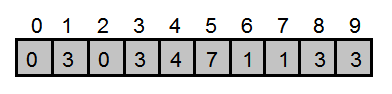
\includegraphics[scale=0.5]{1.png}}
\end{frame}

\begin{frame}[fragile]{Counting Sort Example}
\centerline{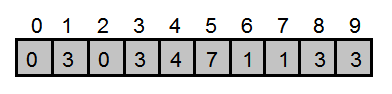
\includegraphics[scale=0.5]{1.png}}

2. Scan the {\tt counts} array so that {\tt counts[i]} contains the number of keys less than {\tt i}.
\begin{lstlisting}
int total = 0;
int c;
for (int j = 0; j < counts.length; j++){
    c = counts[j];
    counts[j] = total;
    total = total + c;
}
\end{lstlisting}
\centerline{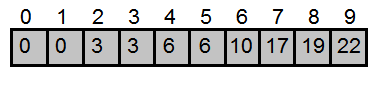
\includegraphics[scale=0.5]{2.png}}
\end{frame}

\begin{frame}[fragile]{Counting Sort Example}
\centerline{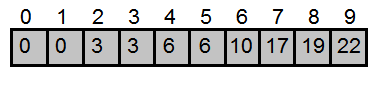
\includegraphics[scale=0.5]{2.png}}

3. Let $s$ be the sorted output array. Walk through array $x$ and copy each item to its final position in $y$. When you copy key $k$, you must increment {\tt counts[k]} to make sure that the next item with key $k$ goes into the next slot.
 {
  \begin{lstlisting}
for (int i = 0; i < arr.length; i += 1){
    y[counts[arr[i]]] = x[i];
    counts[arr[i]] += 1;
}
  \end{lstlisting}
  }
{\tt \small int[] sorted = \{1, 1, 1, 3, 3, 3, 4, 4, 4, 5, 5, 5, 5, 5, 5, 5, 6, 7, 8, 8, 9, 9, 9\}}
\end{frame}

\begin{frame}{What is Radix Sort?}
\begin{itemize}
\item Sort number of buckets $q$ (a.k.a. radix) at one time, from least to most significant.
\item After the most significant radix is sorted, the numbers are completely sorted.
\item This works because counting sort is stable.
\end{itemize}


{\tt int[] arr = \{134, 63, 874, 907, 975, 191, 575, 758, 624, 8, 290, 923, 907, 199, 898, 390, 530, 355, 611, 299\};} \newline \newline
How would this array be sorted using radix sort with $q = 10$ buckets?
\end{frame}

% Hashing %
% ------------------------------------------------------------------------ %
\section{Hashing}
\subsection{Hashing}

\begin{frame}[fragile]{Hash Tables}
\begin{itemize}
\item Stores a set of keys, values
\item Useful because {\tt find} and {\tt add} are constant amortized time
\item Hashcode: used to map a specific key to a bucket in the hashtable
\end{itemize}
\end{frame}

\begin{frame}[fragile]{Hash Tables}

{\tt int[] arr = \{15, 32, 75, 41, 75, 6, 76, 51, 82, 66\};} \newline
 {
  \begin{lstlisting}
int n = 10;
private int hashCode(int i){
    return i % n;
}
  \end{lstlisting}
  }
What would the has table look like with:
\begin{itemize}
\item external chaining?
\item open addressing?
\end{itemize}
\end{frame}

\begin{frame}
  \frametitle{\huge{That's it!}}
\LARGE{Good luck on your midterm and thanks for coming! \newline
Please fill out a feedback form before you leave! \newline
}
\end{frame}



\end{document}

